\documentclass[a4paper,11pt]{article}
\usepackage{tikz}
\usepackage{amsmath,amssymb}
\usepackage{xcolor}
\usepackage{hyperref}
\usepackage{booktabs}
\usepackage{geometry}
\geometry{margin=2.5cm}

\usetikzlibrary{matrix,positioning,arrows.meta,calc}

% Colour definitions matching the CFA channels
\definecolor{cfared}{RGB}{200,60,60}
\definecolor{cfagreen}{RGB}{60,160,60}
\definecolor{cfablue}{RGB}{60,100,200}
\definecolor{cfagrey}{RGB}{180,180,180}

\title{RCD Demosaicing for the Rotated Dufaycolor 4$\times$4 CFA}
\author{}
\date{}

\begin{document}
\maketitle

\begin{abstract}
Dufaycolor was one of the first practical colour-screen photographic
processes, exposing a single panchromatic emulsion through a fine
colour-filter array (CFA) printed on the film base.  Digitising such
material requires demosaicing the raw scan to recover a full-colour
image.  We describe an adaptation of the Ratio Corrected Demosaicing
(RCD) algorithm to a new, rotated 4$\times$4 Dufaycolor CFA geometry
in which the dominant (red) channel forms a standard Bayer-like
checkerboard while the green and blue channels occupy complementary
diagonal strips.  The resulting algorithm reuses the standard RCD
steps for the dominant channel with only minor modifications, and
introduces a novel phase-invariant strip-blend step for the sparse
channels that eliminates the period-4 banding artefact caused by the
asymmetric knight-move neighbourhood of the non-dominant colours.
\end{abstract}

\section{The Dufaycolor Colour-Filter Array}

\subsection{Historical context}

Dufaycolor (1930s--1950s) used a regular reseau of red, green, and blue
filter elements printed at high density directly onto the film base.
Unlike the Bayer CFA of modern digital sensors, the Dufay reseau was not
square-aligned but was formed by overlaying horizontal colour stripes
with a fine ruled grid, giving a characteristic cross-hatch appearance.

When Dufaycolor film is scanned at high resolution the scanner captures
the raw modulated image; a demosaicing step is then required to
reconstruct a conventional RGB image, exactly as is done for digital
camera raw files.

\subsection{The rotated 4$\times$4 pattern}

We work with a computationally convenient rotation of the original
Dufay geometry that places filter boundaries on the integer pixel grid
and achieves 100\% pixel coverage---every demosaiced pixel carries
useful colour information.  Coordinates follow the screen convention
used throughout the code: $x$ increases rightward, $y$ increases
\emph{downward} ($y=0$ is the top row).  The repeating $4\times4$ tile is:

\begin{center}
\begin{small}
\begin{tabular}{c|cccc}
$y\backslash x$ & 0 & 1 & 2 & 3 \\\hline
0 (top)    & G & R & B & R \\
1          & R & B & R & G \\
2          & B & R & G & R \\
3 (bottom) & R & G & R & B \\
\end{tabular}
\end{small}
\end{center}


\begin{center}
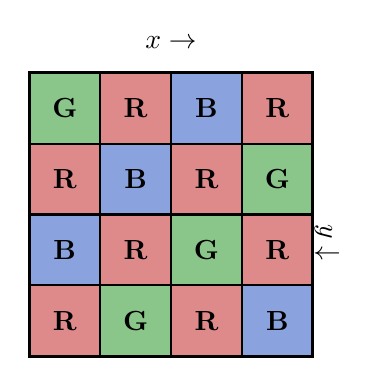
\begin{tikzpicture}[scale=0.9]
  % Screen convention: y=0 at top, y increases downward.
  % TikZ y-axis is inverted: TikZ row (3-y_screen) = y_screen.
  % Screen row 0 (GRBR) at TikZ y=3 (visual top); row 3 (RGRB) at TikZ y=0 (bottom).
  % Screen y=0, TikZ y=3: G R B R
  \fill[cfagreen!60](0,3) rectangle (1,4); \node[font=\bfseries] at (0.5,3.5) {G};
  \fill[cfared!60]  (1,3) rectangle (2,4); \node[font=\bfseries] at (1.5,3.5) {R};
  \fill[cfablue!60] (2,3) rectangle (3,4); \node[font=\bfseries] at (2.5,3.5) {B};
  \fill[cfared!60]  (3,3) rectangle (4,4); \node[font=\bfseries] at (3.5,3.5) {R};
  % Screen y=1, TikZ y=2: R B R G
  \fill[cfared!60]  (0,2) rectangle (1,3); \node[font=\bfseries] at (0.5,2.5) {R};
  \fill[cfablue!60] (1,2) rectangle (2,3); \node[font=\bfseries] at (1.5,2.5) {B};
  \fill[cfared!60]  (2,2) rectangle (3,3); \node[font=\bfseries] at (2.5,2.5) {R};
  \fill[cfagreen!60](3,2) rectangle (4,3); \node[font=\bfseries] at (3.5,2.5) {G};
  % Screen y=2, TikZ y=1: B R G R
  \fill[cfablue!60] (0,1) rectangle (1,2); \node[font=\bfseries] at (0.5,1.5) {B};
  \fill[cfared!60]  (1,1) rectangle (2,2); \node[font=\bfseries] at (1.5,1.5) {R};
  \fill[cfagreen!60](2,1) rectangle (3,2); \node[font=\bfseries] at (2.5,1.5) {G};
  \fill[cfared!60]  (3,1) rectangle (4,2); \node[font=\bfseries] at (3.5,1.5) {R};
  % Screen y=3, TikZ y=0: R G R B
  \fill[cfared!60]  (0,0) rectangle (1,1); \node[font=\bfseries] at (0.5,0.5) {R};
  \fill[cfagreen!60](1,0) rectangle (2,1); \node[font=\bfseries] at (1.5,0.5) {G};
  \fill[cfared!60]  (2,0) rectangle (3,1); \node[font=\bfseries] at (2.5,0.5) {R};
  \fill[cfablue!60] (3,0) rectangle (4,1); \node[font=\bfseries] at (3.5,0.5) {B};
  \draw[thick] (0,0) grid (4,4);
  \draw[very thick] (0,0) rectangle (4,4);
  \node[above] at (2,4.2) {$x\rightarrow$};
  \node[right,rotate=-90] at (4.2,2) {$y\downarrow$};
\end{tikzpicture}
\end{center}

The colour of pixel $(x,y)$ is determined by $s = (x+y)\bmod 4$:
\begin{align}
  s \equiv 1 \text{ or } 3 \pmod{4} &\;\Rightarrow\; \textbf{Red}\quad   (50\%)\label{eq:red}\\
  s \equiv 0 \pmod{4}               &\;\Rightarrow\; \textbf{Green}\quad  (25\%)\label{eq:green}\\
  s \equiv 2 \pmod{4}               &\;\Rightarrow\; \textbf{Blue}\quad   (25\%)\label{eq:blue}
\end{align}

Three structural observations are key to the demosaicing strategy:

\begin{enumerate}
\item \textbf{Red is a Bayer checkerboard.}  The red channel occupies
  every pixel where $x+y$ is odd---exactly the same geometry as green in
  a standard RGGB Bayer sensor.  Its density is 50\% and all four
  cardinal neighbours of any pixel are red.
  
\item \textbf{Green and blue form complementary diagonal strips.}  The
  green strip ($s=0$) and blue strip ($s=2$) run parallel to one another
  along the anti-diagonal direction ($x+y=\text{const}$).  Each has
  density 25\%.  The strips alternate G--R--B--R with period 4 in the
  direction perpendicular to the strip.

\item \textbf{Cardinal neighbourhood of Red pixels.}  From any red pixel, the four nearest
  non-red neighbours are at cardinal distance 1.  Critically, their distribution depends
  on the $(x+y)$ phase of the red pixel:
  \begin{itemize}
    \item Phase $s \equiv 1 \pmod{4}$: Green is at West/North; Blue is at East/South.
    \item Phase $s \equiv 3 \pmod{4}$: Green is at East/South; Blue is at West/North.
  \end{itemize}
  This phase-dependent orientation exactly mirrors the R@G and B@G geometry in a standard Bayer CFA.
\end{enumerate}
\subsection{Strip structure visualised}

\begin{center}
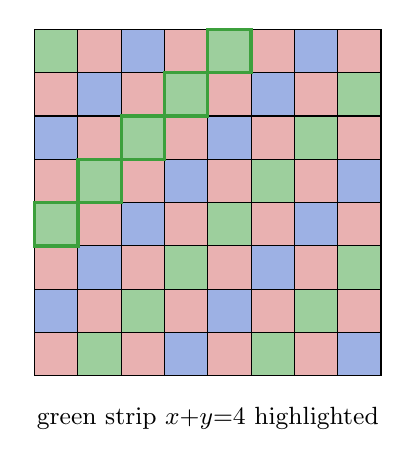
\begin{tikzpicture}[scale=0.55]
  % Screen convention: colour at screen(x,y) = mod(x+y,4).
  % TikZ y_tikz = 7 - y_screen, so s = mod(x + 7 - y_tikz, 4).
  \foreach \x in {0,...,7}
    \foreach \y in {0,...,7}{
      \pgfmathtruncatemacro\s{mod(\x + 7 - \y, 4)}
      \ifcase\s
        \fill[cfagreen!50] (\x,\y) rectangle +(1,1);
      \or
        \fill[cfared!40]   (\x,\y) rectangle +(1,1);
      \or
        \fill[cfablue!50]  (\x,\y) rectangle +(1,1);
      \or
        \fill[cfared!40]   (\x,\y) rectangle +(1,1);
      \fi
    }
  \draw (0,0) grid (8,8);
  % Highlight screen strip x+y_screen=4: y_tikz = x+3
  \foreach \x in {0,...,4}{
    \pgfmathtruncatemacro\yt{\x+3}
    \draw[very thick,cfagreen] (\x,\yt) rectangle +(1,1);
  }
  \node[below,font=\small] at (4,-0.5) {green strip $x{+}y{=}4$ highlighted};
\end{tikzpicture}
\quad
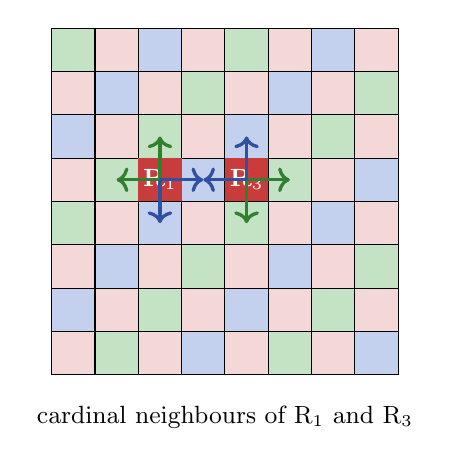
\begin{tikzpicture}[scale=0.55]
  % Background CFA, screen convention: s = mod(x + 7 - y_tikz, 4)
  \foreach \x in {0,...,7}
    \foreach \y in {0,...,7}{
      \pgfmathtruncatemacro\s{mod(\x + 7 - \y, 4)}
      \ifcase\s
        \fill[cfagreen!30] (\x,\y) rectangle +(1,1);
      \or
        \fill[cfared!20]   (\x,\y) rectangle +(1,1);
      \or
        \fill[cfablue!30]  (\x,\y) rectangle +(1,1);
      \or
        \fill[cfared!20]   (\x,\y) rectangle +(1,1);
      \fi
    }
  \draw (0,0) grid (8,8);
  
  % Phase 1 Red pixel: screen(2,3) -> s=(2+3)=5 = 1 mod 4. TikZ y = 7-3 = 4.
  \fill[cfared] (2,4) rectangle (3,5);
  \node[white,font=\bfseries\small] at (2.5,4.5) {R$_1$};
  % Green neighbours (West, North in screen). TikZ y: North is y+1.
  \draw[->,very thick,cfagreen!80!black] (2.5,4.5)--(1.5,4.5); % West
  \draw[->,very thick,cfagreen!80!black] (2.5,4.5)--(2.5,5.5); % North
  % Blue neighbours (East, South in screen). TikZ y: South is y-1.
  \draw[->,very thick,cfablue!80!black] (2.5,4.5)--(3.5,4.5); % East
  \draw[->,very thick,cfablue!80!black] (2.5,4.5)--(2.5,3.5); % South

  % Phase 3 Red pixel: screen(4,3) -> s=(4+3)=7 = 3 mod 4. TikZ y = 7-3 = 4.
  \fill[cfared] (4,4) rectangle (5,5);
  \node[white,font=\bfseries\small] at (4.5,4.5) {R$_3$};
  % Green neighbours (East, South in screen).
  \draw[->,very thick,cfagreen!80!black] (4.5,4.5)--(5.5,4.5); % East
  \draw[->,very thick,cfagreen!80!black] (4.5,4.5)--(4.5,3.5); % South
  % Blue neighbours (West, North in screen).
  \draw[->,very thick,cfablue!80!black] (4.5,4.5)--(3.5,4.5); % West
  \draw[->,very thick,cfablue!80!black] (4.5,4.5)--(4.5,5.5); % North

  \node[below,font=\small] at (4,-0.5) {cardinal neighbours of R$_1$ and R$_3$};
\end{tikzpicture}
\end{center}
\noindent\textit{Left:} 8$\times$8 portion of the CFA; the thick border highlights a single
green strip ($x+y=4$). \textit{Right:} Phase-1 ($R_1$) and Phase-3 ($R_3$) red pixels,
showing their directly adjacent green (green arrows) and blue (blue arrows) cardinal neighbours.

\section{The RCD Algorithm — Background}

Ratio Corrected Demosaicing (RCD) was introduced by Sanz~Rodr\'iguez
\cite{rcd} and is the basis of the demosaicing pipeline in
\textit{darktable}.  For a standard Bayer CFA it proceeds in four steps.

\subsection{Directional discrimination (Step 1)}
A sixth-order high-pass filter (HPF) is applied to the raw CFA values
in both horizontal and vertical directions:
\[
  H_{\rm HPF}(x) = \bigl[f(x-3)-f(x-1)-f(x+1)+f(x+3)\bigr]
                   - 3\bigl[f(x-2)+f(x+2)\bigr] + 6\,f(x).
\]

\begin{center}
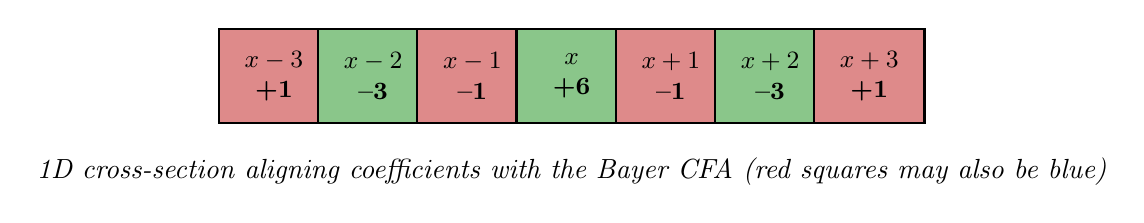
\begin{tikzpicture}[scale=0.9, every node/.style={font=\small}]
  \tikzset{
    pixel/.style={draw, thick, minimum width=1.4cm, minimum height=1.2cm, align=center}
  }
  
  \node[pixel, fill=cfared!60]   (pM3) at (0,0)   {$x-3$\\\textbf{+1}};
  \node[pixel, fill=cfagreen!60] (pM2) at (1.4,0) {$x-2$\\\textbf{--3}};
  \node[pixel, fill=cfared!60]   (pM1) at (2.8,0) {$x-1$\\\textbf{--1}};
  \node[pixel, fill=cfagreen!60] (p0)  at (4.2,0) {$x$\\\textbf{+6}};
  \node[pixel, fill=cfared!60]   (pP1) at (5.6,0) {$x+1$\\\textbf{--1}};
  \node[pixel, fill=cfagreen!60] (pP2) at (7.0,0) {$x+2$\\\textbf{--3}};
  \node[pixel, fill=cfared!60]   (pP3) at (8.4,0) {$x+3$\\\textbf{+1}};

  \node[below=0.3cm of p0, font=\itshape] {1D cross-section aligning coefficients with the Bayer CFA (red squares may also be blue)};
\end{tikzpicture}
\end{center}

The weights of this filter are specifically chosen to compute a robust second-order discrete derivative (a Laplacian) that perfectly cancels out linear colour gradients by leveraging data from both colour channels simultaneously. 

Because of the CFA layout, the filter decomposes into two independent parts:
\begin{itemize}
    \item \textbf{The Green part:} The coefficients on the green pixels are $-3$, $+6$, $-3$. Factoring out $-3$, we get $-3 \times [f(x-2) - 2f(x) + f(x+2)]$, which is exactly $-3 \nabla^2 G(x)$ applied to the green sub-grid.
    \item \textbf{The Red/Blue part:} The coefficients on the red (or blue) pixels are $+1$, $-1$, $-1$, $+1$. These can be rearranged into $[f(x-3) - 2f(x-1) + f(x+1)] + [f(x-1) - 2f(x+1) + f(x+3)]$, which is the sum of two adjacent 2nd derivatives: $\nabla^2 R(x-1) + \nabla^2 R(x+1)$.
\end{itemize}

A foundational assumption in demosaicing is that the colour difference ($R - G$) is locally constant across structural edges, implying $\nabla^2 R \approx \nabla^2 G$. Assuming the second derivative is relatively smooth locally, the sum of the adjacent red derivatives approximates $2 \nabla^2 G(x)$. Thus, the complete filter evaluates to:
\[
    H_{\rm HPF}(x) \approx 2 \nabla^2 G(x) - 3 \nabla^2 G(x) = -\nabla^2 G(x)
\]
Because the coefficients for each colour channel independently sum to zero, the filter perfectly rejects flat areas and smooth linear colour gradients, responding purely to high-frequency structural edges. This makes the resulting directional discrimination highly robust against colour noise and chromatic aberration.

The squared magnitudes of these HPF responses are accumulated over a local 3-pixel window to improve statistical robustness. The ratio of these accumulated energies gives a \emph{VH direction weight} $\alpha\in[0,1]$:
\[
  \alpha = \frac{E_V}{E_V + E_H}, \qquad
  \alpha\approx 1 \Rightarrow \text{prefer H estimate},\quad
  \alpha\approx 0 \Rightarrow \text{prefer V estimate}.
\]
In the implementation, this weight is further refined by comparing the local pixel's discrimination against the average of its four diagonal neighbors, ensuring that directional decisions are spatially consistent and less sensitive to single-pixel noise.

\subsection{Step 2 — Low-pass filter (LPF)}
At each non-dominant pixel, a luminance estimate is computed by summing the $3\times3$ CFA neighbourhood with weights $1, \tfrac12, \tfrac14$ for centre, cardinal, and diagonal neighbours respectively. Crucially, in the implementation, this LPF value is **only calculated and stored at non-dominant (Red or Blue) sites**, serving as a sparse normalisation reference for the dominant channel recovery in Step 3. At dominant (Green) sites, the LPF value is zeroed and unused.

\begin{center}
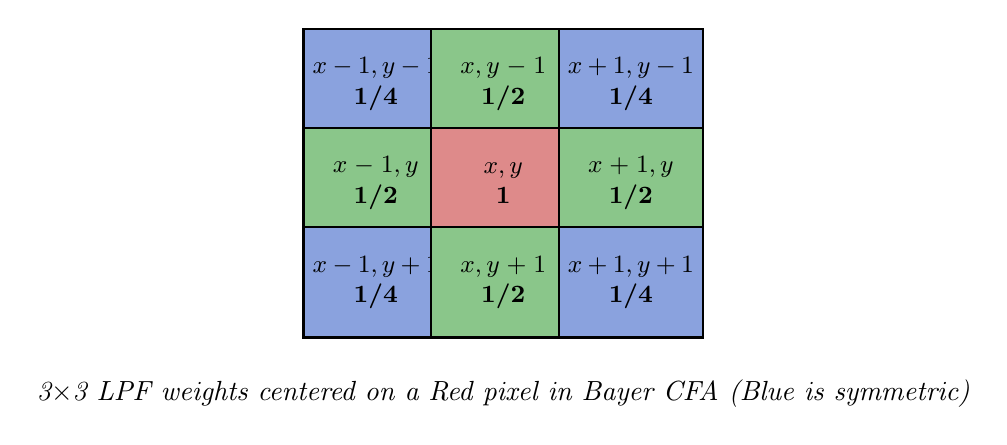
\begin{tikzpicture}[scale=0.9, every node/.style={font=\small}]
  \tikzset{
    pixel/.style={draw, thick, text width=1.6cm, minimum height=1.4cm, align=center}
  }
  
  % Top row
  \node[pixel, fill=cfablue!60]   (pNW) at (0, 2.8)   {$x-1, y-1$\\\textbf{1/4}};
  \node[pixel, fill=cfagreen!60]  (pN)  at (1.8, 2.8) {$x, y-1$\\\textbf{1/2}};
  \node[pixel, fill=cfablue!60]   (pNE) at (3.6, 2.8) {$x+1, y-1$\\\textbf{1/4}};
  
  % Middle row
  \node[pixel, fill=cfagreen!60]  (pW)  at (0, 1.4)   {$x-1, y$\\\textbf{1/2}};
  \node[pixel, fill=cfared!60]    (pC)  at (1.8, 1.4) {$x, y$\\\textbf{1}};
  \node[pixel, fill=cfagreen!60]  (pE)  at (3.6, 1.4) {$x+1, y$\\\textbf{1/2}};
  
  % Bottom row
  \node[pixel, fill=cfablue!60]   (pSW) at (0, 0)     {$x-1, y+1$\\\textbf{1/4}};
  \node[pixel, fill=cfagreen!60]  (pS)  at (1.8, 0)   {$x, y+1$\\\textbf{1/2}};
  \node[pixel, fill=cfablue!60]   (pSE) at (3.6, 0)   {$x+1, y+1$\\\textbf{1/4}};

  \node[below=0.4cm of pS, font=\itshape] {3$\times$3 LPF weights centered on a Red pixel in Bayer CFA (Blue is symmetric)};
\end{tikzpicture}
\end{center}

\subsection{Step 3 — Dominant channel at non-dominant sites}
The dominant channel (green in Bayer) is estimated by \emph{ratio-corrected} cardinal interpolation. The directional blending is steered by high-fidelity gradients that measure variation up to 4 pixels deep. For each cardinal direction (e.g., North), the gradient is defined as:
\begin{align*}
    G_N &= \epsilon + |f(x, y-1) - f(x, y+1)| \\
        &+ |f(x, y) - f(x, y-2)| \\
        &+ |f(x, y-1) - f(x, y-3)| \\
        &+ |f(x, y-2) - f(x, y-4)|
\end{align*}
These gradients are used for cross-gradient weighting:
\[
    \hat{G}_V = \frac{G_S \cdot \hat{G}_N + G_N \cdot \hat{G}_S}{G_N + G_S}
\]
where $\hat{G}_N = G_N \cdot \frac{2\,L_0}{L_0 + L_{-2}}$ is the ratio-corrected estimate. The final value is obtained by blending the vertical and horizontal estimates using the refined $\alpha$ discriminant:
\[
  \hat G = \alpha\,\hat G_H + (1-\alpha)\,\hat G_V.
\]

\begin{center}
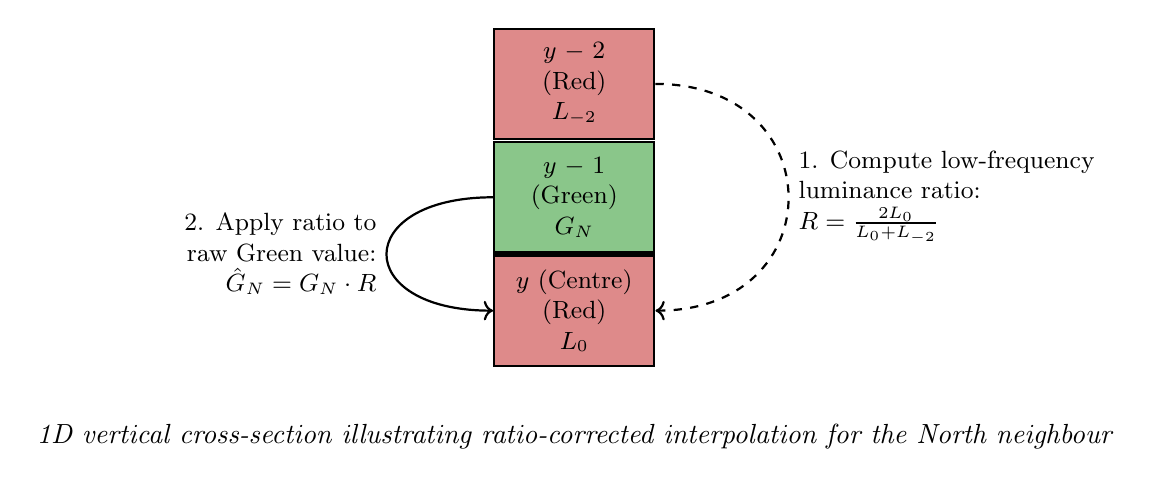
\begin{tikzpicture}[scale=0.9, every node/.style={font=\small}]
  \tikzset{
    pixel/.style={draw, thick, text width=1.8cm, minimum height=1.4cm, align=center}
  }
  
  \node[pixel, fill=cfared!60]   (pN2) at (0, 3.2)  {$y-2$\\(Red)\\\textbf{$L_{-2}$}};
  \node[pixel, fill=cfagreen!60] (pN1) at (0, 1.6)  {$y-1$\\(Green)\\\textbf{$G_N$}};
  \node[pixel, fill=cfared!60]   (pC)  at (0, 0)    {$y$ (Centre)\\(Red)\\\textbf{$L_0$}};
  
  \draw[->, thick, dashed] (pN2.east) .. controls +(2.5,0) and +(2.5,0) .. node[right, align=left] {1. Compute low-frequency \\ luminance ratio:\\$R = \frac{2 L_0}{L_0 + L_{-2}}$} (pC.east);
  
  \draw[->, thick] (pN1.west) .. controls +(-2,0) and +(-2,0) .. node[left, align=right] {2. Apply ratio to \\ raw Green value:\\$\hat{G}_N = G_N \cdot R$} (pC.west);

  \node[below=0.6cm of pC, font=\itshape] {1D vertical cross-section illustrating ratio-corrected interpolation for the North neighbour};
\end{tikzpicture}
\end{center}

\textbf{Logic of Ratio Correction:} 
The straightforward way to interpolate the missing green value at the red centre ($y$) using its north neighbour ($y-1$) would be to simply copy $G_N$, or average $G_N$ and $G_S$. However, this ignores the local luminance gradient. 
By calculating the low-pass filter (LPF) values at the non-dominant pixels ($L_0$ at $y$ and $L_{-2}$ at $y-2$), the algorithm can sense the luminance trend. The term $\frac{L_0 + L_{-2}}{2}$ represents the expected low-frequency luminance at the position of the green pixel ($y-1$). 
The ratio $\frac{L_0}{(L_0 + L_{-2})/2}$ therefore represents how much brighter or darker the centre pixel is compared to its surrounding neighbourhood. By multiplying the raw green value $G_N$ by this ratio, the interpolation perfectly preserves local luminance gradients and avoids colour fringing at structural edges.

\subsection{Step 4 — Non-dominant channels}
The missing red and blue values are recovered in two sub-steps:
\begin{itemize}
  \item \emph{Step 4.2 — R@B and B@R} using diagonal color-difference interpolation weighted by the PQ discriminant.
  \item \emph{Step 4.3 — R@G and B@G} using cardinal color-difference interpolation weighted by the VH discriminant.
\end{itemize}
In both cases, the already-reconstructed Green channel is used as the structural guide.

\begin{center}
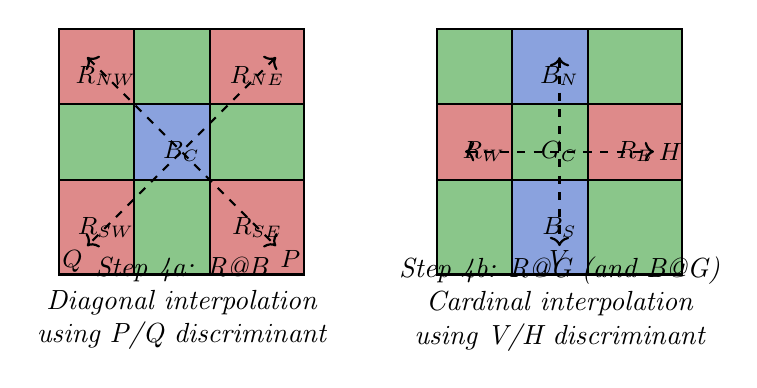
\begin{tikzpicture}[scale=0.8, every node/.style={font=\small}]
  \tikzset{
    pixel/.style={draw, thick, minimum width=1.2cm, minimum height=1.2cm, align=center}
  }
  
  % Left figure: Step 4a (R@B)
  \begin{scope}[xshift=0cm]
    \node[pixel, fill=cfared!60]   at (0, 2.4) {$R_{NW}$};
    \node[pixel, fill=cfagreen!60] at (1.2, 2.4) {};
    \node[pixel, fill=cfared!60]   at (2.4, 2.4) {$R_{NE}$};
    
    \node[pixel, fill=cfagreen!60] at (0, 1.2) {};
    \node[pixel, fill=cfablue!60]  (B) at (1.2, 1.2) {$B_C$};
    \node[pixel, fill=cfagreen!60] at (2.4, 1.2) {};
    
    \node[pixel, fill=cfared!60]   at (0, 0) {$R_{SW}$};
    \node[pixel, fill=cfagreen!60] at (1.2, 0) {};
    \node[pixel, fill=cfared!60]   at (2.4, 0) {$R_{SE}$};

    \draw[<->, thick, dashed] (-0.3, 2.7) -- (2.7, -0.3) node[below right=-3pt] {$P$};
    \draw[<->, thick, dashed] (2.7, 2.7) -- (-0.3, -0.3) node[below left=-3pt] {$Q$};
    
    \node[below=0.6cm of B, font=\itshape, align=center] {Step 4a: R@B \\ Diagonal interpolation \\ using P/Q discriminant};
  \end{scope}

  % Right figure: Step 4b (R@G)
  \begin{scope}[xshift=6cm]
    \node[pixel, fill=cfagreen!60] at (0, 2.4) {};
    \node[pixel, fill=cfablue!60]  at (1.2, 2.4) {$B_N$};
    \node[pixel, fill=cfagreen!60] at (2.4, 2.4) {};
    
    \node[pixel, fill=cfared!60]   at (0, 1.2) {$R_W$};
    \node[pixel, fill=cfagreen!60] (G) at (1.2, 1.2) {$G_C$};
    \node[pixel, fill=cfared!60]   at (2.4, 1.2) {$R_E$};
    
    \node[pixel, fill=cfagreen!60] at (0, 0) {};
    \node[pixel, fill=cfablue!60]  at (1.2, 0) {$B_S$};
    \node[pixel, fill=cfagreen!60] at (2.4, 0) {};

    \draw[<->, thick, dashed] (-0.3, 1.2) -- (2.7, 1.2) node[right=-2pt] {$H$};
    \draw[<->, thick, dashed] (1.2, 2.7) -- (1.2, -0.3) node[below=-2pt] {$V$};
    
    \node[below=0.6cm of G, font=\itshape, align=center] {Step 4b: R@G (and B@G)\\ Cardinal interpolation \\ using V/H discriminant};
  \end{scope}
\end{tikzpicture}
\end{center}

\textbf{Logic of Non-Dominant Channel Recovery:} \\
Once the dominant Green channel is fully populated, it acts as a high-fidelity structural guide for the missing Red and Blue channels. 

\textbf{Step 4a (R@B and B@R):} To interpolate Red at a Blue pixel, the four diagonal Red neighbours are used. A new diagonal discriminant ($P$ vs.\ $Q$) is computed to detect whether the structure flows along the NW--SE or NE--SW diagonal. The Red values are then blended along the chosen diagonal, and ratio-corrected using the now fully known Green channel (e.g., $R_{NW} \cdot \frac{G_C}{G_{NW}}$) to preserve sharp details.

\textbf{Step 4b (R@G and B@G):} To interpolate Red at a Green pixel, the adjacent cardinal Red neighbours are used (which lie either horizontally or vertically depending on the Bayer phase). Because the distance is only 1 pixel, simple colour-difference interpolation is sufficient. The algorithm calculates the colour differences ($R-G$) at the neighbours, blends them according to the existing $V/H$ discriminant from Step 1, and adds the result to the central Green value: $\hat{R}_C = G_C + \Delta(R-G)_{\rm blend}$. This perfectly reconstructs edges without chromatic aberration.

\subsection{Diagonal Directional Discrimination ($P/Q$)}

The squared magnitudes of diagonal 6th-order HPFs are accumulated over a local 3-pixel window, and the ratio gives a \emph{PQ direction weight} analogous to the VH weight in Step 1. This steers the diagonal interpolation to follow the primary structural flow. In Step 4.2, the estimate along a diagonal (e.g., $P$) is computed as a weighted average of color differences ($\Delta = C - G$) at diagonal neighbors:
\[
    \hat{\Delta}_P = \frac{nw\_grad \cdot \Delta_{SE} + se\_grad \cdot \Delta_{NW}}{nw\_grad + se\_grad}
\]
where the gradients use the same 4-pixel deep logic as in Step 3. The final color value is $\hat{C} = G_C + \text{blend}(\hat{\Delta}_P, \hat{\Delta}_Q)$.

\begin{center}
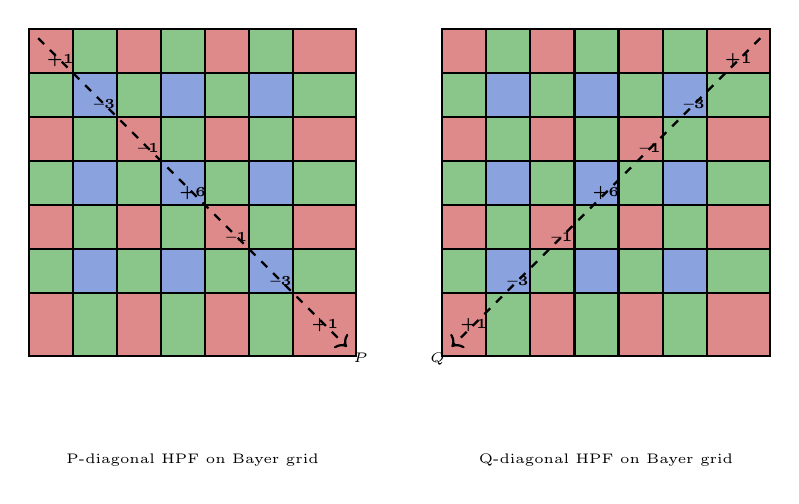
\begin{tikzpicture}[scale=0.7, every node/.style={font=\tiny}]
  \tikzset{
    pixel/.style={draw, thick, minimum width=0.8cm, minimum height=0.8cm, align=center}
  }
  
  % P-diagonal (NW-SE)
  \begin{scope}[xshift=0cm]
    \foreach \y in {-3,...,3} {
      \foreach \x in {-3,...,3} {
        \pgfmathparse{int(abs(mod(\x+\y,2))) == 1 ? "cfagreen!60" : (int(abs(mod(\x,2))) == 1 ? "cfared!60" : "cfablue!60")}
        \edef\fillcol{\pgfmathresult}
        \node[pixel, fill=\fillcol] (P\x\y) at (\x*0.8, -\y*0.8) {};
      }
    }
    \node at (P-3-3) {\textbf{+1}}; \node at (P-2-2) {\textbf{--3}}; \node at (P-1-1) {\textbf{--1}};
    \node at (P00)   {\textbf{+6}};   \node at (P11)   {\textbf{--1}}; \node at (P22)   {\textbf{--3}};
    \node at (P33)   {\textbf{+1}};
    \draw[->, thick, dashed] (-3.5*0.8, 3.5*0.8) -- (3.5*0.8, -3.5*0.8) node[below right=-2pt] {$P$};
    \node[below=3.2cm] at (0,0) {P-diagonal HPF on Bayer grid};
  \end{scope}

  % Q-diagonal (NE-SW)
  \begin{scope}[xshift=7.5cm]
    \foreach \y in {-3,...,3} {
      \foreach \x in {-3,...,3} {
        \pgfmathparse{int(abs(mod(\x+\y,2))) == 1 ? "cfagreen!60" : (int(abs(mod(\x,2))) == 1 ? "cfared!60" : "cfablue!60")}
        \edef\fillcol{\pgfmathresult}
        \node[pixel, fill=\fillcol] (Q\x\y) at (\x*0.8, -\y*0.8) {};
      }
    }
    \node at (Q3-3) {\textbf{+1}}; \node at (Q2-2) {\textbf{--3}}; \node at (Q1-1) {\textbf{--1}};
    \node at (Q00)   {\textbf{+6}};   \node at (Q-11)  {\textbf{--1}}; \node at (Q-22)  {\textbf{--3}};
    \node at (Q-33)  {\textbf{+1}};
    \draw[->, thick, dashed] (3.5*0.8, 3.5*0.8) -- (-3.5*0.8, -3.5*0.8) node[below left=-2pt] {$Q$};
    \node[below=3.2cm] at (0,0) {Q-diagonal HPF on Bayer grid};
  \end{scope}
\end{tikzpicture}
\end{center}


\section{RCD for the Dufay $4\times4$ Reseau}

The Dufaycolor $4\times4$ reseau presents a fundamentally different geometry compared to the classic Bayer pattern. To facilitate the adaptation of the RCD algorithm, we establish a direct mapping between the Bayer components and the Dufay elements based on their topological roles:

\begin{center}
\begin{tabular}{lll}
\toprule
\textbf{Role} & \textbf{Bayer CFA} & \textbf{Dufay CFA} \\
\midrule
Dominant Channel & Green (50\%, Checkerboard) & \textbf{Red} (50\%, Checkerboard) \\
Non-Dominant A & Red (25\%, Square grid) & \textbf{Green} (25\%, Diagonal strip) \\
Non-Dominant B & Blue (25\%, Square grid) & \textbf{Blue} (25\%, Diagonal strip) \\
\bottomrule
\end{tabular}
\end{center}

Because the dominant Red channel retains the checkerboard topology, the early stages of the RCD pipeline translate almost perfectly by substituting Red for the standard Green guide. The significant divergence occurs in the final stages when reconstructing the non-dominant Green and Blue channels, as their sparse layout breaks the symmetric $3\times3$ neighbourhoods.

\subsection{Directional Discrimination (Step 1)}
The $V/H$ and $P/Q$ discriminants are calculated on the raw CFA data. Because Red is the dominant checkerboard, the $6^{\text{th}}$-order HPF is applied primarily to the Red channel to measure structural gradients, mirroring Step 1 of standard RCD.

\subsubsection{Cardinal Discriminants ($V/H$)}
In the Dufay $4\times4$ reseau, any horizontal or vertical line through a Red pixel alternates between Red and a non-dominant color (either Green or Blue). For example, a horizontal line through an $R_1$ pixel ($s=1$) follows the sequence $G, R, B, R, G, \dots$. 

As in standard Bayer RCD, the $6^{\text{th}}$-order HPF is specifically designed to cancel linear color differences between the dominant and non-dominant channels. In the Dufay pattern, this cancellation is only mathematically robust when the filter is **centered on a Red (dominant) pixel**.

In this case, the non-dominant neighbors at $x\pm1$ and $x\pm3$ always contain a balanced pair of Green and Blue samples (due to the anti-diagonal stagger). Evaluating $H_{\rm HPF}$ centered on a Red pixel yields:
\begin{align*}
    H_{\rm HPF}(x) &= [G(x-3) - B(x-1) - B(x+1) + G(x+3)] \\
                   &- 3[R(x-2) + R(x+2)] + 6R(x)
\end{align*}
Assuming $\nabla^2 G \approx \nabla^2 B \approx \nabla^2 R$, the terms in the first bracket sum to zero at structural edges, isolating the structural Laplacian of the Red channel. 

Conversely, when the filter is **centered on a non-dominant (Green or Blue) pixel**, the heavy coefficients ($-3, +6, -3$) fall on a mix of dominant and non-dominant samples, making it impossible to reject the color-filter modulation without knowing the already reconstructed values. The implementation therefore restricts the directional discrimination pass exclusively to the Red checkerboard sites.

\begin{center}
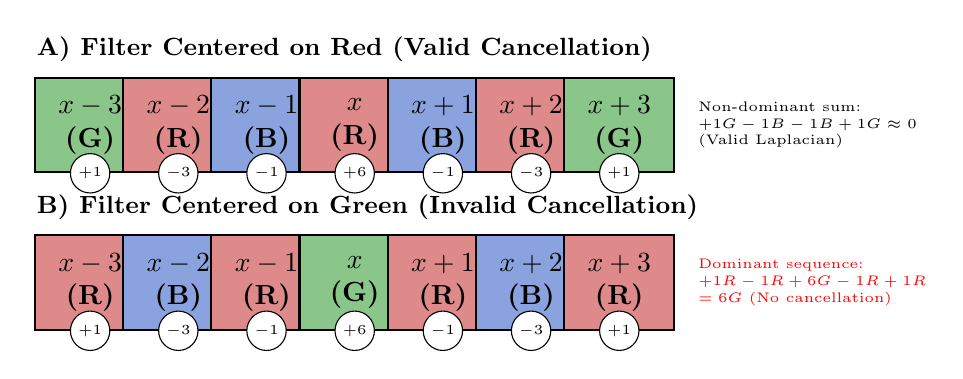
\begin{tikzpicture}[scale=0.8, every node/.style={font=\tiny}]
  \tikzset{
      pixel/.style={draw, thick, minimum width=1.4cm, minimum height=1.2cm, align=center, font=\bfseries},
      weight/.style={circle, draw, fill=white, inner sep=1pt, font=\tiny\bfseries, minimum size=0.5cm}
  }
  
  \begin{scope}[yshift=2.5cm]
      \node[anchor=west, font=\small\bfseries] at (-1, 1.2) {A) Filter Centered on Red (Valid Cancellation)};
      \node[pixel, fill=cfagreen!60] (p0) at (0, 0)   {$x-3$\\(G)};
      \node[pixel, fill=cfared!60]   (p1) at (1.4, 0) {$x-2$\\(R)};
      \node[pixel, fill=cfablue!60]  (p2) at (2.8, 0) {$x-1$\\(B)};
      \node[pixel, fill=cfared!60]   (p3) at (4.2, 0) {$x$\\(R)};
      \node[pixel, fill=cfablue!60]  (p4) at (5.6, 0) {$x+1$\\(B)};
      \node[pixel, fill=cfared!60]   (p5) at (7.0, 0) {$x+2$\\(R)};
      \node[pixel, fill=cfagreen!60] (p6) at (8.4, 0) {$x+3$\\(G)};
      
      \node[weight] at (p0.south) {$+1$}; \node[weight] at (p1.south) {$-3$};
      \node[weight] at (p2.south) {$-1$}; \node[weight] at (p3.south) {$+6$};
      \node[weight] at (p4.south) {$-1$}; \node[weight] at (p5.south) {$-3$};
      \node[weight] at (p6.south) {$+1$};
      
      \node[anchor=west, align=left] at (9.5, 0) {Non-dominant sum:\\$+1G - 1B - 1B + 1G \approx 0$\\(Valid Laplacian)};
  \end{scope}
  
  \begin{scope}[yshift=0cm]
      \node[anchor=west, font=\small\bfseries] at (-1, 1.2) {B) Filter Centered on Green (Invalid Cancellation)};
      \node[pixel, fill=cfared!60]   (q0) at (0, 0)   {$x-3$\\(R)};
      \node[pixel, fill=cfablue!60]  (q1) at (1.4, 0) {$x-2$\\(B)};
      \node[pixel, fill=cfared!60]   (q2) at (2.8, 0) {$x-1$\\(R)};
      \node[pixel, fill=cfagreen!60] (q3) at (4.2, 0) {$x$\\(G)};
      \node[pixel, fill=cfared!60]   (q4) at (5.6, 0) {$x+1$\\(R)};
      \node[pixel, fill=cfablue!60]  (q5) at (7.0, 0) {$x+2$\\(B)};
      \node[pixel, fill=cfared!60]   (q6) at (8.4, 0) {$x+3$\\(R)};
      
      \node[weight] at (q0.south) {$+1$}; \node[weight] at (q1.south) {$-3$};
      \node[weight] at (q2.south) {$-1$}; \node[weight] at (q3.south) {$+6$};
      \node[weight] at (q4.south) {$-1$}; \node[weight] at (q5.south) {$-3$};
      \node[weight] at (q6.south) {$+1$};
      
      \node[anchor=west, align=left, text=red] at (9.5, 0) {Dominant sequence:\\$+1R - 1R + 6G - 1R + 1R$\\$ = 6G$ (No cancellation)};
  \end{scope}
\end{tikzpicture}
\end{center}

Critically, the phase of the red pixel determines whether the cardinal neighbors are Green (H) and Blue (V) or vice versa. The implementation calculates the directional energies $E_H$ and $E_V$ at each Red site and accumulates them using a local window. This accumulation is weighted based on the local neighborhood to prioritize valid Red-centered gradients.

\begin{center}
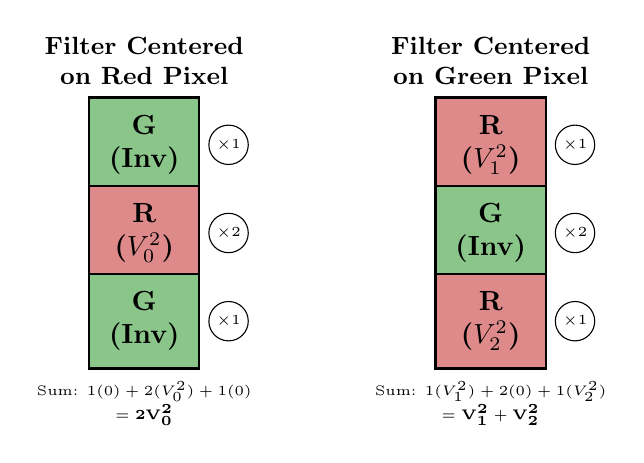
\begin{tikzpicture}[scale=0.8, every node/.style={font=\tiny}]
  \tikzset{
      pixel/.style={draw, thick, minimum width=1.4cm, minimum height=1.2cm, align=center, font=\bfseries},
      weight/.style={circle, draw, fill=white, inner sep=1pt, font=\tiny\bfseries, minimum size=0.5cm}
  }
  
  \begin{scope}[xshift=0cm]
      \node[anchor=south, font=\small\bfseries, align=center] at (0, 2.2) {Filter Centered\\on Red Pixel};
      \node[pixel, fill=cfagreen!60] (p0) at (0, 1.4)  {G\\(Inv)};
      \node[pixel, fill=cfared!60]   (p1) at (0, 0)    {R\\($V^2_0$)};
      \node[pixel, fill=cfagreen!60] (p2) at (0, -1.4) {G\\(Inv)};
      \node[weight, right=0.1cm of p0] (w0) {$\times 1$};
      \node[weight, right=0.1cm of p1] (w1) {$\times 2$};
      \node[weight, right=0.1cm of p2] (w2) {$\times 1$};
      \node[anchor=north, align=center] at (0, -2.2) {Sum: $1(0) + 2(V^2_0) + 1(0)$\\$ = \mathbf{2 V^2_0}$};
  \end{scope}
  
  \begin{scope}[xshift=5.5cm]
      \node[anchor=south, font=\small\bfseries, align=center] at (0, 2.2) {Filter Centered\\on Green Pixel};
      \node[pixel, fill=cfared!60]   (q0) at (0, 1.4)  {R\\($V^2_1$)};
      \node[pixel, fill=cfagreen!60] (q1) at (0, 0)    {G\\(Inv)};
      \node[pixel, fill=cfared!60]   (q2) at (0, -1.4) {R\\($V^2_2$)};
      \node[weight, right=0.1cm of q0] (w0_2) {$\times 1$};
      \node[weight, right=0.1cm of q1] (w1_2) {$\times 2$};
      \node[weight, right=0.1cm of q2] (w2_2) {$\times 1$};
      \node[anchor=north, align=center] at (0, -2.2) {Sum: $1(V^2_1) + 2(0) + 1(V^2_2)$\\$ = \mathbf{V^2_1 + V^2_2}$};
  \end{scope}
\end{tikzpicture}
\end{center}

\subsubsection{Dufay Diagonal Asymmetry ($P/Q$)}
In the Dufay $4\times4$ reseau, the diagonal lines exhibit asymmetric behavior due to the staggered $G/B$ strips. 

\begin{itemize}
    \item \textbf{Anti-diagonal Direction ($Q$):} This direction ($x+y=\text{const}$) aligns perfectly with the color strips. Any line in this direction is \textbf{monochromatic} (either all-Red, all-Green, or all-Blue). 
    \item \textbf{Main Diagonal Direction ($P$):} This direction ($x-y=\text{const}$) crosses the strips. There are two distinct cases for the color sequence:
    \begin{itemize}
        \item \textbf{All-Red:} Lines where $x-y$ is odd consist entirely of Red samples.
        \item \textbf{Alternating Non-Dominant:} Lines where $x-y$ is even strictly alternate between Green and Blue: $G, B, G, B, \dots$.
    \end{itemize}
\end{itemize}

Crucially, the $6^{\text{th}}$-order HPF only cancels color differences when centered on a Red pixel in an alternating sequence (like standard Bayer $R, G, R, B$). In the Dufay $P$-direction, the $G/B$ alternating lines \emph{contain no Red pixels}. Thus, the HPF cannot be evaluated on those lines. The implementation therefore restricts the HPF evaluation to the Red checkerboard pixels ($x+y$ is odd), ensuring that every computed gradient is either monochromatic or a valid Red-centered alternating sequence.

\begin{center}
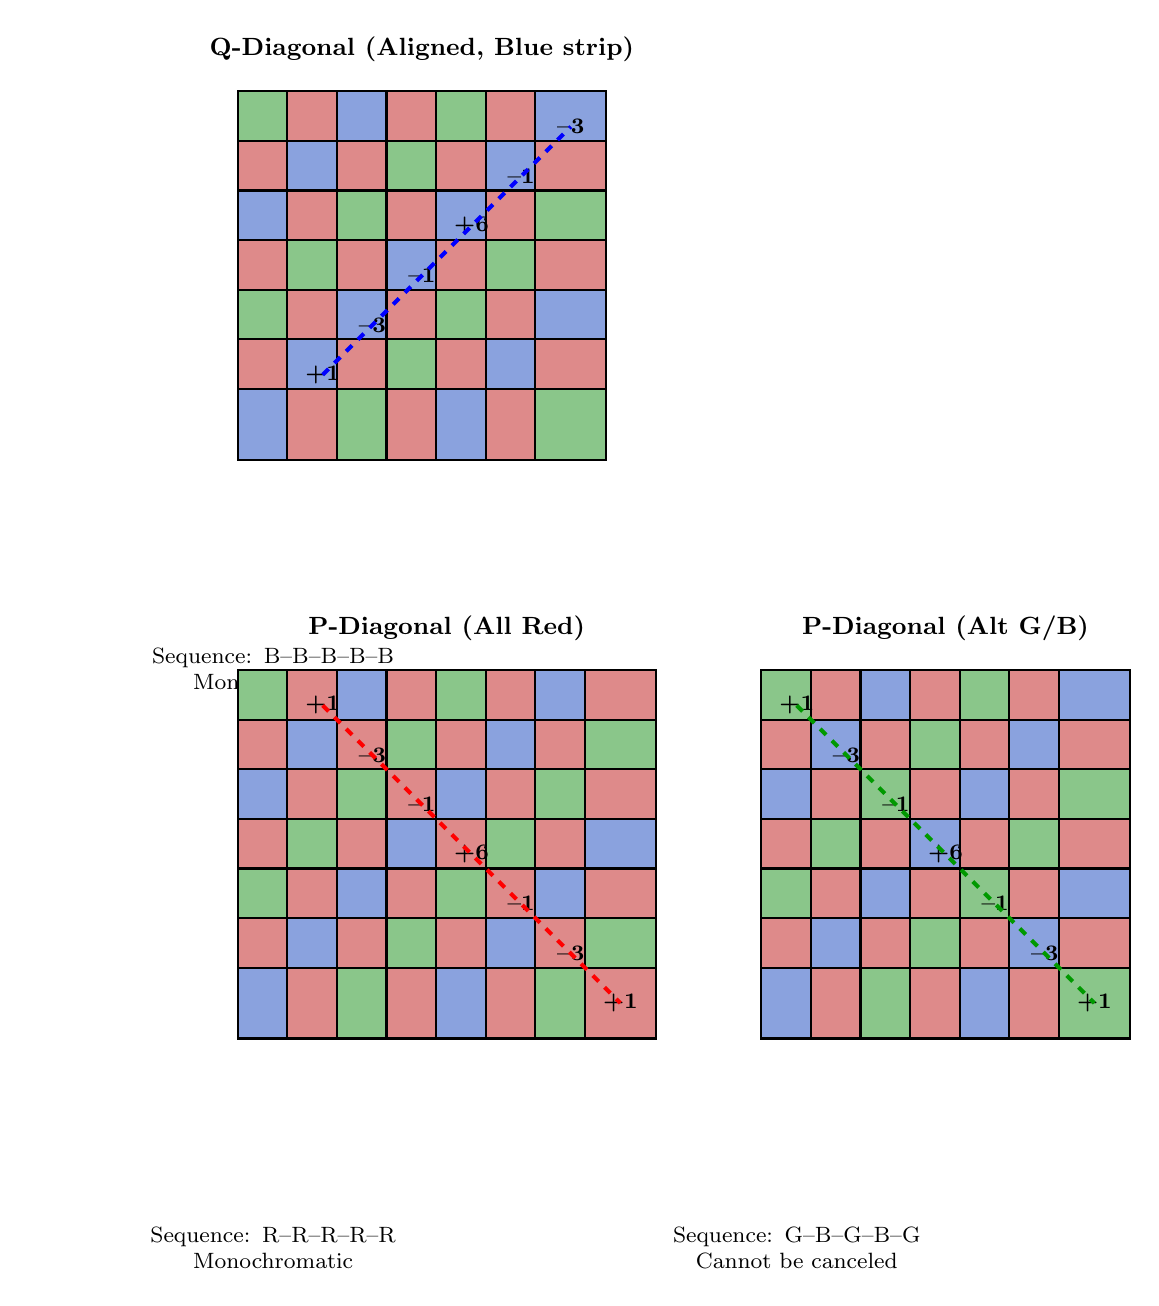
\begin{tikzpicture}[scale=0.7, every node/.style={font=\footnotesize}]
  \tikzset{
    pixel/.style={draw, thick, minimum width=0.9cm, minimum height=0.9cm, align=center}
  }

  % --- ROW 1: Q-Diagonal (Anti-diagonal) ---
  \begin{scope}[yshift=0cm]
    \node[anchor=south, font=\small\bfseries] at (2.7, 1.0) {Q-Diagonal (Aligned, Blue strip)};
    \foreach \y in {0,...,6} {
      \foreach \x in {0,...,6} {
        \pgfmathsetmacro{\s}{int(mod(\x+\y,4))}
        \ifcase\s \edef\fillcol{cfagreen!60} \or \edef\fillcol{cfared!60} \or \edef\fillcol{cfablue!60} \or \edef\fillcol{cfared!60} \fi
        \node[pixel, fill=\fillcol] (Q\x\y) at (\x*0.9, -\y*0.9) {};
      }
    }
    % Q-Diagonal weights. Center (4,2) s=2(Blue). 
    \node at (Q15) {\textbf{+1}}; \node at (Q24) {\textbf{--3}}; \node at (Q33) {\textbf{--1}};
    \node at (Q42) {\textbf{+6}};
    \node at (Q51) {\textbf{--1}}; \node at (Q60) {\textbf{--3}};
    \draw[blue, line width=1.5pt, dashed] (Q15.center) -- (Q60.center);
    \node[below=6.5cm, align=center, text width=6cm] {Sequence: B--B--B--B--B\\Monochromatic};
  \end{scope}

  % --- ROW 2: P-Diagonal Case 1 (All Red) ---
  \begin{scope}[yshift=-10.5cm, xshift=0cm]
    \node[anchor=south, font=\small\bfseries] at (3.15, 1.0) {P-Diagonal (All Red)};
    \foreach \y in {0,...,6} {
      \foreach \x in {0,...,7} {
        \pgfmathsetmacro{\s}{int(mod(\x+\y,4))}
        \ifcase\s \edef\fillcol{cfagreen!60} \or \edef\fillcol{cfared!60} \or \edef\fillcol{cfablue!60} \or \edef\fillcol{cfared!60} \fi
        \node[pixel, fill=\fillcol] (P1\x\y) at (\x*0.9, -\y*0.9) {};
      }
    }
    % P-Diagonal weights (All Red). Center (4,3) s=3(Red).
    \node at (P110) {\textbf{+1}}; \node at (P121) {\textbf{--3}}; \node at (P132) {\textbf{--1}};
    \node at (P143) {\textbf{+6}};
    \node at (P154) {\textbf{--1}}; \node at (P165) {\textbf{--3}}; \node at (P176) {\textbf{+1}};
    \draw[red, line width=1.5pt, dashed] (P110.center) -- (P176.center);
    \node[below=6.5cm, align=center, text width=6cm] {Sequence: R--R--R--R--R\\Monochromatic};
  \end{scope}

  % --- ROW 2: P-Diagonal Case 2 (Alt G/B) ---
  \begin{scope}[yshift=-10.5cm, xshift=9.5cm]
    \node[anchor=south, font=\small\bfseries] at (2.7, 1.0) {P-Diagonal (Alt G/B)};
    \foreach \y in {0,...,6} {
      \foreach \x in {0,...,6} {
        \pgfmathsetmacro{\s}{int(mod(\x+\y,4))}
        \ifcase\s \edef\fillcol{cfagreen!60} \or \edef\fillcol{cfared!60} \or \edef\fillcol{cfablue!60} \or \edef\fillcol{cfared!60} \fi
        \node[pixel, fill=\fillcol] (P2\x\y) at (\x*0.9, -\y*0.9) {};
      }
    }
    % P-Diagonal weights (Alt G/B). Center (3,3) s=2(Blue).
    \node at (P200) {\textbf{+1}}; \node at (P211) {\textbf{--3}}; \node at (P222) {\textbf{--1}};
    \node at (P233) {\textbf{+6}};
    \node at (P244) {\textbf{--1}}; \node at (P255) {\textbf{--3}}; \node at (P266) {\textbf{+1}};
    \draw[green!60!black, line width=1.5pt, dashed] (P200.center) -- (P266.center);
    \node[below=6.5cm, align=center, text width=6cm] {Sequence: G--B--G--B--G\\Cannot be canceled};
  \end{scope}
\end{tikzpicture}
\end{center}

\subsection{Low-Pass Filter (Step 2)}

In Step 2, a local luminance estimate $L$ is computed to facilitate ratio-corrected interpolation. 

\subsubsection{Cardinal 3x3 LPF}
At each non-dominant (Green or Blue) site, a local luminance estimate $L$ is computed using a $3\times3$ cardinal neighborhood. In the Dufay $4\times4$ reseau, a key geometric property is that the cardinal neighbors of any non-dominant pixel are \textbf{all Red}. This provides a highly robust and uniform luma reference for ratio correction, as the dominant channel is sampled at every adjacent position.

\begin{center}
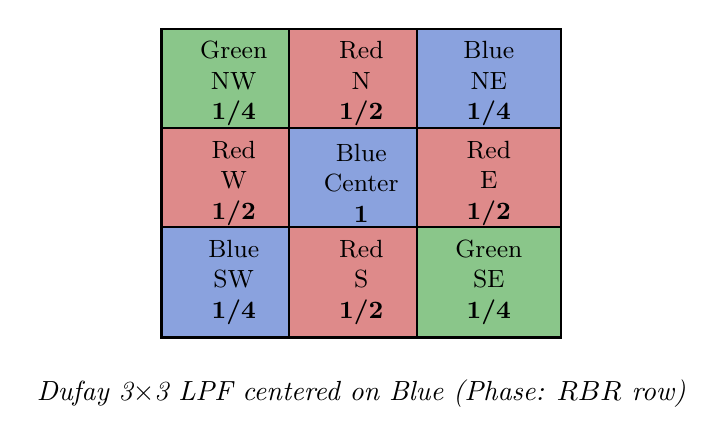
\begin{tikzpicture}[scale=0.9, every node/.style={font=\small}]
  \tikzset{
    pixel/.style={draw, thick, text width=1.6cm, minimum height=1.4cm, align=center}
  }
  
  % Grid: GRB / RBR / BRG (centered on Blue RBR)
  % Top row
  \node[pixel, fill=cfagreen!60]   (pNW) at (0, 2.8)   {Green\\NW\\\textbf{1/4}};
  \node[pixel, fill=cfared!60]     (pN)  at (1.8, 2.8) {Red\\N\\\textbf{1/2}};
  \node[pixel, fill=cfablue!60]    (pNE) at (3.6, 2.8) {Blue\\NE\\\textbf{1/4}};
  
  % Middle row
  \node[pixel, fill=cfared!60]     (pW)  at (0, 1.4)   {Red\\W\\\textbf{1/2}};
  \node[pixel, fill=cfablue!60]    (pC)  at (1.8, 1.4) {Blue\\Center\\\textbf{1}};
  \node[pixel, fill=cfared!60]     (pE)  at (3.6, 1.4) {Red\\E\\\textbf{1/2}};
  
  % Bottom row
  \node[pixel, fill=cfablue!60]    (pSW) at (0, 0)     {Blue\\SW\\\textbf{1/4}};
  \node[pixel, fill=cfared!60]     (pS)  at (1.8, 0)   {Red\\S\\\textbf{1/2}};
  \node[pixel, fill=cfagreen!60]   (pSE) at (3.6, 0)   {Green\\SE\\\textbf{1/4}};

  \node[below=0.4cm of pS, font=\itshape] {Dufay 3$\times$3 LPF centered on Blue (Phase: $RBR$ row)};
\end{tikzpicture}
\end{center}

The LPF value at $(x,y)$ is computed as:
\[
    L(x,y) = f(x,y) + 0.5 \sum f_{\text{cardinal}} + 0.25 \sum f_{\text{diagonal}}
\]
This estimate is used as the normalization reference in Step 3 to preserve sharp structural detail while avoiding color fringing.

\subsection{Dominant Channel Recovery (Step 3)}

The goal of Step 3 is to interpolate the dominant \textbf{Red} channel at all non-dominant (Green and Blue) locations. 

\subsubsection{Ratio-Corrected Cardinal Interpolation}
The algorithm uses the $V/H$ discriminant computed in Step 1 to blend between horizontal and vertical ratio-corrected estimates. For a sparse pixel (Green or Blue) at $(x,y)$, the vertical estimate $\hat{R}_V$ is:
\[
    \hat{R}_V = f(x,y-1) \cdot \frac{2 \cdot L(x,y)}{L(x,y) + L(x,y-2)}
\]
where $f(x,y-1)$ is a raw Red sample and $L$ is the $3\times3$ LPF value calculated at Red sites at distance 2.

\begin{center}
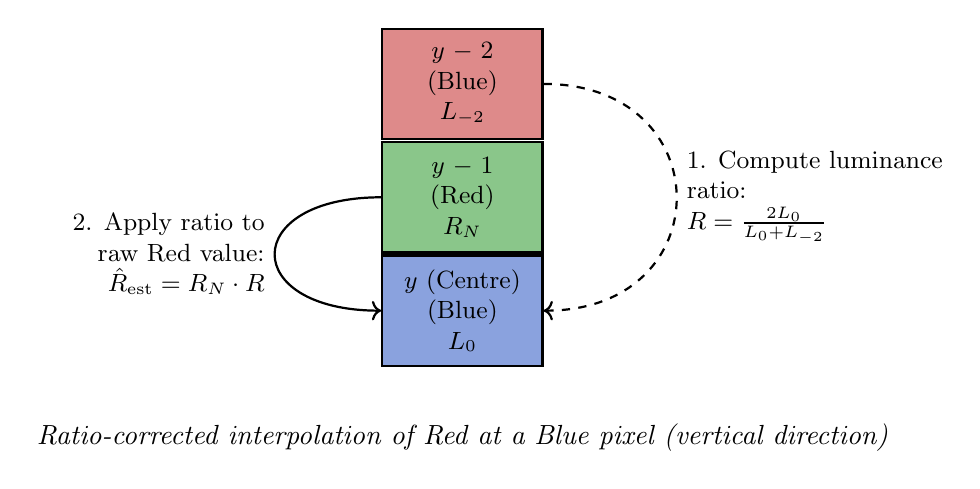
\begin{tikzpicture}[scale=0.9, every node/.style={font=\small}]
  \tikzset{
    pixel/.style={draw, thick, text width=1.8cm, minimum height=1.4cm, align=center}
  }
  
  \node[pixel, fill=cfared!60]   (pN2) at (0, 3.2)  {$y-2$\\(Blue)\\\textbf{$L_{-2}$}};
  \node[pixel, fill=cfagreen!60] (pN1) at (0, 1.6)  {$y-1$\\(Red)\\\textbf{$R_N$}};
  \node[pixel, fill=cfablue!60]  (pC)  at (0, 0)    {$y$ (Centre)\\(Blue)\\\textbf{$L_0$}};
  
  \draw[->, thick, dashed] (pN2.east) .. controls +(2.5,0) and +(2.5,0) .. node[right, align=left] {1. Compute luminance \\ ratio:\\$R = \frac{2 L_0}{L_0 + L_{-2}}$} (pC.east);
  
  \draw[->, thick] (pN1.west) .. controls +(-2,0) and +(-2,0) .. node[left, align=right] {2. Apply ratio to \\ raw Red value:\\$\hat{R}_{\rm est} = R_N \cdot R$} (pC.west);

  \node[below=0.6cm of pC, font=\itshape] {Ratio-corrected interpolation of Red at a Blue pixel (vertical direction)};
\end{tikzpicture}
\end{center}

\subsection{Non-Dominant Channel Recovery (Step 4)}

Every pixel now has a reconstructed Red value. In Step 4, we recover the missing Green and Blue values using the Red channel as a structural guide.

\subsubsection{Step 4.2: Missing sparse channels (Green/Blue) at sparse sites}
This step populates the Green channel at Blue pixels and the Blue channel at Green pixels. Because these non-dominant channels form sparse diagonal strips, they only have same-color neighbors along the anti-diagonals. The algorithm calculates diagonal color-difference estimates ($\Delta = C - R$) steered by the $P/Q$ discriminants, using the fully recovered Red channel as the structural guide.

\begin{center}
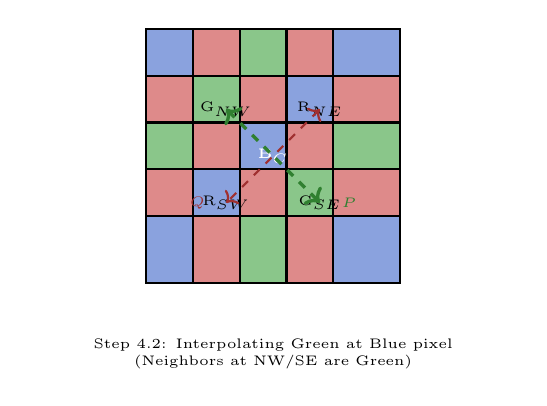
\begin{tikzpicture}[scale=0.7, every node/.style={font=\tiny}]
  \tikzset{
    pixel/.style={draw, thick, minimum width=0.85cm, minimum height=0.85cm, align=center}
  }
  
  % Step 4.2 Diagram: G at B site
  \foreach \y in {-2,...,2} {
    \foreach \x in {-2,...,2} {
      % center (0,0) s=10 mod 4 = 2 (Blue)
      \pgfmathsetmacro{\s}{int(mod(\x+\y+10,4))}
      \ifcase\s \edef\fillcol{cfagreen!60} \or \edef\fillcol{cfared!60} \or \edef\fillcol{cfablue!60} \or \edef\fillcol{cfared!60} \fi
      \node[pixel, fill=\fillcol] (N\x\y) at (\x*0.85, -\y*0.85) {};
    }
  }
  
  \node[white] at (N00) {\bf B$_C$};
  \node at (N-1-1) {G$_{NW}$};
  \node at (N11)   {G$_{SE}$};
  \node at (N1-1)  {R$_{NE}$};
  \node at (N-11)  {R$_{SW}$};

  \draw[<->, very thick, cfagreen!80!black, dashed] (N-1-1.center) -- (N11.center) node[right=4pt] {$P$};
  \draw[<->, thick, cfared!80!black, dashed] (N1-1.center) -- (N-11.center) node[left=4pt] {$Q$};

  \node[below=2.2cm, align=center, text width=6cm] {Step 4.2: Interpolating Green at Blue pixel\\(Neighbors at NW/SE are Green)};
\end{tikzpicture}
\end{center}

The algorithm calculates diagonal estimates of the **color difference** $\Delta = (C - R)$ steered by the $P/Q$ discriminants (where $C$ is Green or Blue). Although only one diagonal contains raw samples for the target color, the estimate along the other diagonal is still computed using the fully populated Red channel and the reconstructed values from neighboring tiles.

The color-difference estimate along the $P$ diagonal is:
\[
    \hat{\Delta}_{P} = \frac{nw\_grad \cdot \Delta_{SE} + se\_grad \cdot \Delta_{NW}}{nw\_grad + se\_grad}
\]
where $\Delta = C - R$ at the diagonal neighbors. Finally, the missing color value is recovered by adding the blended color difference to the central Red value:
\[
    \hat{C} = R_C + pq\_disc \cdot \hat{\Delta}_Q + (1 - pq\_disc) \cdot \hat{\Delta}_P
\]
The directional weight $pq\_disc$ is near 1 when the structure is aligned with the monochromatic $Q$ diagonal (the strips), ensuring that the interpolation follows the physical geometry of the Dufay reseau.

\subsubsection{Step 4.3: Sparse channels at Red sites (Cardinal)}
To interpolate Green and Blue at Red sites, the cardinal neighbors are used. 

\begin{center}
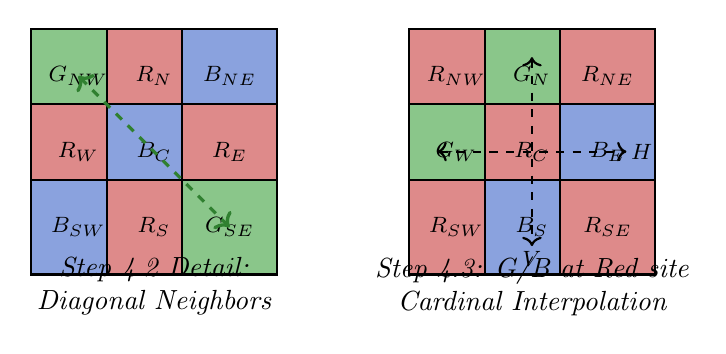
\begin{tikzpicture}[scale=0.8, every node/.style={font=\footnotesize}]
  \tikzset{
    pixel/.style={draw, thick, minimum width=1.2cm, minimum height=1.2cm, align=center}
  }
  
  % Left figure: Step 4.3 (Green at Blue site - restored but renamed)
  \begin{scope}[xshift=0cm]
    \node[pixel, fill=cfagreen!60] (NW) at (0, 2.4) {$G_{NW}$};
    \node[pixel, fill=cfared!60]   at (1.2, 2.4) {$R_N$};
    \node[pixel, fill=cfablue!60]  at (2.4, 2.4) {$B_{NE}$};
    
    \node[pixel, fill=cfared!60]   at (0, 1.2) {$R_W$};
    \node[pixel, fill=cfablue!60]  (B) at (1.2, 1.2) {$B_C$};
    \node[pixel, fill=cfared!60]   at (2.4, 1.2) {$R_E$};
    
    \node[pixel, fill=cfablue!60]  at (0, 0) {$B_{SW}$};
    \node[pixel, fill=cfared!60]   at (1.2, 0) {$R_S$};
    \node[pixel, fill=cfagreen!60] (SE) at (2.4, 0) {$G_{SE}$};

    \draw[<->, very thick, cfagreen!80!black, dashed] (NW.center) -- (SE.center);
    
    \node[below=0.6cm of B, font=\itshape, align=center] {Step 4.2 Detail:\\Diagonal Neighbors};
  \end{scope}

  % Right figure: Step 4.3 (Cardinal)
  \begin{scope}[xshift=6cm]
    \node[pixel, fill=cfared!60]   at (0, 2.4) {$R_{NW}$};
    \node[pixel, fill=cfagreen!60] at (1.2, 2.4) {$G_N$};
    \node[pixel, fill=cfared!60]   at (2.4, 2.4) {$R_{NE}$};
    
    \node[pixel, fill=cfagreen!60] at (0, 1.2) {$G_W$};
    \node[pixel, fill=cfared!60]   (R) at (1.2, 1.2) {$R_C$};
    \node[pixel, fill=cfablue!60]  at (2.4, 1.2) {$B_E$};
    
    \node[pixel, fill=cfared!60]   at (0, 0) {$R_{SW}$};
    \node[pixel, fill=cfablue!60]  at (1.2, 0) {$B_S$};
    \node[pixel, fill=cfared!60]   at (2.4, 0) {$R_{SE}$};

    \draw[<->, thick, dashed] (-0.3, 1.2) -- (2.7, 1.2) node[right=-2pt] {$H$};
    \draw[<->, thick, dashed] (1.2, 2.7) -- (1.2, -0.3) node[below=-2pt] {$V$};
    
    \node[below=0.6cm of R, font=\itshape, align=center] {Step 4.3: G/B at Red site\\Cardinal Interpolation};
  \end{scope}
\end{tikzpicture}
\end{center}

\begin{thebibliography}{9}
\bibitem{rcd} L.~Sanz~Rodr\'iguez, \textit{Ratio Corrected Demosaicing},
  release 2.3, 2011.
\end{thebibliography}

\end{document}
